\documentclass{article}
\usepackage[utf8]{inputenc}
\usepackage[brazil]{babel}
\usepackage{fancyvrb}
\usepackage[alf]{abntex2cite}
\usepackage{graphicx}

\title{
  Analizo: ferramenta livre e extensível para análise estática de código-fonte
}

\author{Joenio Marques da Costa\\
  {\small joenio@joenio.me}
}

\begin{document}

\maketitle

{\it Este artigo é uma tradução livre e atualizada do artigo ``Analizo: an
extensible multi-language source code analysis and visualization toolkit''
\cite{Terceiro2010Analizo} publicado no Congresso Brasileiro de Software:
Teoria e Prática.}

\section{Introdução}

Nós apresentamos o Analizo, um conjunto de ferramentas para análise de código-fonte
e visualização, desenvolvida com os objetivos de ter suporte a múltiplas linguagens,
ser software livre, e ser extensível.

Um outro requisito é que seja capaz de lidar com código-fonte que não compila mais.
Por exemplo, código-fonte com erro de sintaxe ou que referenciam bibliotecas não mais
disponíveis, ou que usa bibliotecas que mudou a API. Isto é importante para poder analisar
código legado em estudos sobre evolução de software.

\section{Arquitetura}

A arquitetura do Analizo apresentada na Figura \ref{arquitetura-analizo},
usando {\it Layered Style} \cite{Clements2002}. Cada camada no diagrama usa
apenas os serviços oferecidos pela camada diretamente abaixo.

\begin{figure}[h]
\center
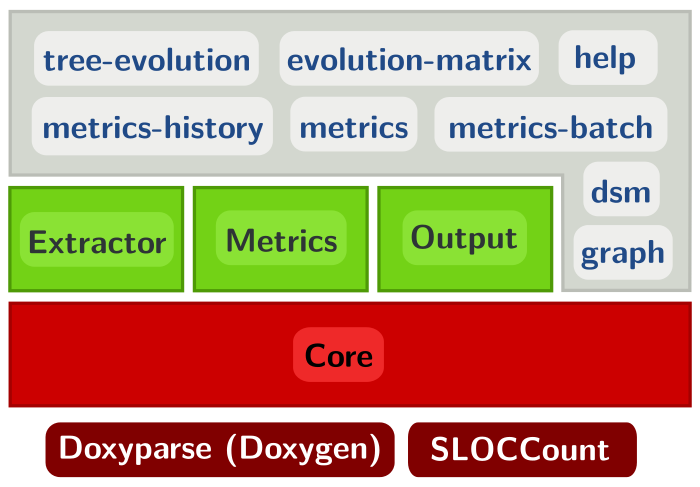
\includegraphics[scale=0.4]{analizo-architecture.png}
\caption{Arquitetura do Analizo, usando Layered Style \cite{Clements2002}}
\label{arquitetura-analizo}
\end{figure}

O {\it Core} contém as estruturas de dados usadas para armazenar informações
a respeito do código-fonte sendo analisado, como a lista de módulos, elementos
dentro de cada módulo (atributos, variáveis, métodos, funções), informações de
depdendencia (chamada, herança, etc). Esta camada implementa a maior parte da lógica
de negócio do Analizo, e não depende de nenhuma outra camada.

A camada {\it Extractor} lida com as informaçoes de código-fonte obtidas pelas
diferenças estratégias presente no Analizo. Os extratores pegam informaçoes do código-fonte
e armazenam estruturas de dados na camada {\it Core}. Isto requer apenas a criação
de uma nova subclasse para adicionar um novo tipo de extrator que faz interface
com outra ferramenta externa ou provendo sua própria análise diretamente.
Atualmente, existem dois extratores. Ambos fazem interface com ferramentas externas
de análise estática de código-fonte:

\begin{itemize}
  \item Analizo::Extractors::Doxyparse é uma interface para o Doxyparse, um parser
        de código-fonte para C, C++ e Java desenvolvida por nosso grupo de pesquisa\cite{Costa2009}.
        Doxyparse é baseado no Doxygen, um sistema de documentação multi-linguagem
  \item Analizo::Extractors::Sloccount é uma interface para o Sloccount desenvolvido por
        David A. Wheeler, uma ferramenta que calcula o número efetivo de linhas de código.
\end{itemize}

As outras camadas intermediárias são {\it Metrics} e {\it Output}. A camada {\it Metrics}
processa as estruturas de dados do {\it Core} para calcular métricas. Até o momento Analizo
suporta um conjunto razoável de métricas (listadas na Seção ???). A camada {\it Output} é
responsável por lidar com diferentes formatos de arquivos. Atualmente, apenas o formato DOT
é implementado no Analizo para representar grafo de dependencia, mas adicionar novos formatos
é simplesmente adicionar novas classes.

A camada {\it Tools} fornece um conjunto de ferramentas de linha de comando que constituem
a interface do analizo, tanto para usuários finais quanto para aplicações de mais alto nível.
Estas ferramentas usam serviços providos pelas outras camadas: eles instanciam as estruturas
de dados do {\it core}, um ou mais extratores, opcionalmente o processador de métricas, um
módulo de formato de saída, e gerencia eles para prover o resultado desejado. A maioria das
funcionalidades descritas na Secao 4 sao implementadas como Analizo tools.

Estas ferramentas sao pensadas na filosofia UNIX: fazem uma tarefa especializada e gera saída
que pode ser utilizada como entrada de outras ferramentas, seja do proprio Analizo ou de ferramentas
externas. Alguma das ferramentas implementadas sobre outras ao inves de manipular explicitamente
os internos do Analizo, e alguns sao desenhads para prover saida para aplicacoes externas como 
programas para desenho de grafos ou visualização de dados.

\section{Funcionalidades}

\subsection{Análise de código-fonte multi-linguagem}

Atualmente Analizo suporta análise de código-fonte escrito em C, C++ e Java. Entretanto,
pode ser estendido para suportar outras linguagens desde que use Doxyparse, que é baseado
no Doxygen e também suporta inúmeras outras linguagens.

\subsection{Métricas}

Analizo reporta tanto métricas em nível de projeto, que é calculada para todo o projeto,
quanto métricas em nível de módulos/classes, que é calculado individualmente para cada módulo.
No nível de projeto, Analizo também provê estatística descritiva básica para cada métrica em
nível de módulo: soma, média, mediana, moda, desvio padrão, variância, skewness e kurtosis da
distribuição, mínimo, e maximo valores. As seguintes métricas são suportadas até o momento:

Project-level metrics: Total Coupling Factor, Total Lines of Code, Total number
of methods per abstract class, Total Number of Modules/Classes, Total number
of modules/classes with at least one defined attributes, Total number of mod-
ules/classes with at least one defined method, Total Number of Methods.

Module-level metrics: Afferent Connections per Class, Average Cyclomatic Com-
plexity per Method, Average Method LOC, Average Number of Parameters per
Method, Coupling Between Objects, Depth of Inheritance Tree, Lack of Cohesion
of Methods, Lines of Code, Max Method LOC, Number of Attributes, Number of
Children, Number of Methods, Number of Public Attributes, Number of Public
Methods, Response For a Class.

\subsection{Métricas e processamento em lote}

A maioria dos estudos quantitativos em Engenharia de Software envolve aquisição de
métricas de código-fonte de um grande número de projetos, processar cada projeto
individualmente é pouco prático, passível de erros e difícil de repetir. Analizo pode processar
multiplos projetos em lote e produzir arquivo de dados CSV com métricas de cada projeto,
bem como um resumo com as métricas em nível de projeto de todos os projetos. Estes
arquivos de dados podem ser facilmente importados em ferramentas de estatística ou planilhas para
análise futura. Pode também ser usado para analizar várias versões de um mesmo projeto,
em estudos sobre evolução de software.

\subsection{Histórico de métricas}

Algumas vezes pesquisadores precisam processar o histórico de projetos de software de
uma forma mais escalável. Analizo pode processar o repositório  de controle de versão e
procer arquivo de dados CSV com valores de métricas para cada revisão onde o código-fonte
foi alterado no projeto. Git e Subversion repositórios são suportados diretamente, repositórios
CVS  devem ser convertidos para Git antes de forma manual.

\subsection{Saída para grafo de dependencia}

Analizo pode gerar saída com informações sobre dependencia entre as entidades do projeto
em um formato adequado para processamento pelas ferramentas de desenho de grafo do Graphviz.
A Figura ? apresenta um exemplo de grafo desenhado pela ferramenta dot do Graphviz a partir
da saída gerada pelo Analizo.

\subsection{Matriz de evolução}

Outra funcionalidade útil do Analizo é gerar matrizes de evolução \ref{Lanza2001}. Após
processar cada release de um projeto (ver Seção ??), o usuário pode solicitar criação
de uma matrix de evolução a partir de arquivos de dados individuais. A Figura ?? apresenta um
exemplo de uma matrix produzida pelo Analizo.

\subsection{Matriz de estrutura de projeto}

Uma funcionalidade recente do Analizo é uma representação visual do
relacionamento entre os módulos do projeto em forma de uma {\it Design
Structure Matrix} (Matriz de estrutura de projeto) \cite{Maccormack2006}, uma
DSM é a representação de um grafo de dependência em forma de uma matriz
quadrada. Um exemplo na Figura ?.

\section{Uso em trabalhos de pesquisa}

Analizo tem sido extensivamente usada por nosso grupo de pesquisa para suportar
projetos de pesquisa:

\begin{itemize}

\item \cite{Amaral2009} usou o grafo de dependencia gerado pelo Analizo para
gerar uma matriz de evolução em um estudo de caso com o projeto VLC.

\item \cite{Costa2009} fez uma comparação entre diferentes estratégias para
extração de informação de dependencias entre módulos do código-fonte,
resultando no desenvolvimento do Doxyparse - o extrator baseado no Doxygen do
Analizo.

\item \cite{Terceiro2009} usou métricas em um estudo exploratório sobre a
evolução da complexidade estrutural em projetos de software livre escritos em
C.

\item \cite{Morais2009} usou a ferramenta de métricas do Analizo como backend
para o Kalibro, um software paraavaliação de métricas.

\item \cite{Terceiro2010} usou o processamento de histórico de métricas para
analizar a história completa de mudanças em 7 projetos de servidor web de
diferentes tamanhos.

\item \cite{Meirelles2010} usou o processamento em lote do Analizo para
processas o código-fonte de mais de 6000 projetos de software livre do
repositório Sourceforge.net.

\item \cite{Meirelles2011} usou o Analizo em um estudo sobre impacto de
métricas de código-fonte na atratividade de projetos de softwares livres.

\item \cite{Terceiro2012Understanding} usou o Analizo para investigar fatores
que influenciam na evolução da complexidade estrutural em projetos de software
livres.

\item \cite{Silva2012} usou o Analizo para minerar 16000 revisões de
repositórios de projetos de software para investigar o potencil de uma nova
métrica chamada Lack of Concern-based Cohesion.

\item \cite{Ronaldo2015} utilizou o Analizo para extrair métricas de
código-fonte de 14 versões da API do sistema Android.

\end{itemize}

A maioria destes trabalhos contribuíram com melhorias para o Analizo, fazendo
ainda mais apropriado para pesquisas envolvendo análise de código-fonte.

\section{Considerações finais}

Este artigo apresenta o Analizo, um conjunto de ferramentas para análise e visualização
de código-fonte com suporta a C, C++ e Java. Analizo é útil tanto para pesquisadores
trabalhando com análise de código-fonte quanto para profissionais que precisama analisar
seu código para identificar problemas potenciais ou melhorias.

Analizo é software livre, licenciado sob a GNU General Public License versão
3. Seu código-fonte, bem como pacotes binários, manuais e tutoriais podem ser
obtidas em http://analizo.org. Todas as ferramentas são auto-documentadas e podem
ser consultadas como páginas de manual UNIX. Analizo é escrito em Perl.

\bibliography{bibliografia}
\appendix

\end{document}
